\chapter{Electro-optical topology optimization problems}\label{chap:eo}
%\section{Electro-optical systems~\cite{ownpub4}}\label{sec:electro_optical}
Electro-optics describes the interaction between electricity and optics. Electricity involves the presence and flow of electric charges, which can generate electromagnetic fields (\eqref{eq:faraday}--\eqref{eq:Gauss_B}).
However, the main difference between electricity and optics is that the frequency of the electrical fields ($\omega_E$)
is much lower than for optical fields ($\omega_E \ll \omega $), so that they can generally be treated as static fields\footnote{Similarly, as discussed in \secref{sec:nanophotonics}, the size ($s$) of optical devices
is usually much smaller than the wavelength of the electrical fields ($s\ll \lambda_E $), and the field is effectively quasistatic.}.
The interaction between electricity and optics is used in a variety of technologies such as high-speed modulators for optical communications~\cite{modu, modu1, modu2, pockels}, switches~\cite{eo_switch}, electrically pumped lasers~\cite{laser,laser_pic}, and integrated photonic circuits~\cite{laser_pic}. 
These systems exploit mechanisms ranging from the electro-optic effect~\cite{eo_effect} to carrier-induced refractive index
 changes~\cite{c_i_n} to achieve efficient light manipulation and generation, bridging electro-optic principles with carrier-driven processes central to optoelectronics.

As a basic example of electro-optic coupling, one can consider the \textbf{electro-optic effect}\footnote{This is analogous to the thermo-optic effect presented in \secref{sec:to_effect}.}~\cite{eo_effect},
where the refractive index of a material ($n$) can be modified under the influence of an external (static) electric field. The linear term in the electro-optic effect is known as the
Pockels effect $
    \Delta n = -(1/2) n^3 r E\,,$
where $r$ is the electro-optic coefficient, and $E$ is the applied electric field~\cite{pockels}. The quadratic term 
is the electro-optic Kerr effect $\Delta n = n_2 E^2$, where $n_2$ is the Kerr-coefficient~\cite{phot_crys}. Note that based on the applied external
quasistatic electric field, one can model the refractive index change by accounting for higher order terms in the expansion of the polarizability
in terms of the electric field (\eqref{eq:polarization}), where the Pockels effect corresponds to the $\chi^{(2)}$ term, and the Kerr effect to the $\chi^{(3)}$ term.

Topology optimization provides a powerful, systematic framework for designing electro-optical devices and has already been widely adopted in other coupled-electrical systems, such as electromechanical~\cite{MEMS_multi,electrostatic_act} or electrochemical~\cite{electrode} systems. However, electro-optics remains relatively unexplored, with only a few studies, such as~\cite{g_heat}, which focuses on diffusion-based designs for carrier dynamics in semiconductor devices.

In the remainder of the chapter, we focus on our work~\cite{ownpub4}, in which we apply topology 
optimization to design a nanolaser device, where electrical pumping can be used to achieve efficient light emission.

\section{Topology optimization of nanolasers~\cite{ownpub4}}\label{sec:laser}

\subsection*{A figure of merit for nanolaser performance}

A nanolaser is a nanoscale device that emits light by stimulating the emission of photons in a gain medium, which is typically a semiconductor material. This is illustrated
in \figref{fig:laser2d}~(a), where a pump laser excites the emitters or carriers (e.g., electrons and holes) in a gain medium $D_0$, which then emits light into an output channel (e.g., waveguide) via
stimulated emission. This physical
mechanism can be described using the Maxwell-Bloch equations~\cite{haken_laser_dynamics, PhysRev.134.A1429, SALT_original}, which are a set of nonlinear time-dependent 
partial differential equations. When aligned to a high-quality-factor ($Q \sim$ lifetime/period)~\cite{phot_crys} lasing mode ($Q\gtrapprox 100$~\cite{cerjan_2016}), the Maxwell-Bloch equations can be simplified via the single-pole approximation (SPA-) steady-state ab-initio laser theory (SALT)~\cite{Ge_2010}, leading to
\begin{equation}\label{eq:SPA_SALT}
    \left[(\nabla \times 
     \nabla \times ) -\left[\varepsilon_c(\mathbf{r})-i \Delta \varepsilon^{\prime \prime} (\mathbf{r})\right] \left(\frac{\omega_L}{c}\right)^2\right] \mathbf{E}_L(\mathbf{r})=0\,,
\end{equation}
where $\mathbf{E}_L$ is the lasing mode, $\omega_L$ is the lasing frequency, $\varepsilon_c$ is the dielectric permittivity of the passive (no gain) cavity, and the change in the 
imaginary part of the permittivity is given by
\begin{equation}\label{eq:gain_SALT}
        \Delta \varepsilon^{\prime \prime} (\mathbf{r}) =  \frac{D_0(\mathbf{r}) d_\text{pump}}{1+ e_c^{-2}\left|\mathbf{E}_L(\mathbf{r})\right|^2}\,,
\end{equation}
where $D_0$ is the gain profile, $d_\text{pump}$ is a scalar pumping strength, and $e_c$ is a non-dimensionalization parameter~\cite{Ge_2010}. While the SPA-SALT model (\eqref{eq:SPA_SALT}) 
is simpler and can be solved more efficiently than the Maxwell-Bloch equations, it still requires one to solve a nonlinear eigenproblem. This can be computationally expensive, especially in 
inverse design tasks where hundreds or thousands of such problems must be solved to optimize a device.

\begin{figure}[tb]
    \centering
    \makebox[\textwidth][c]{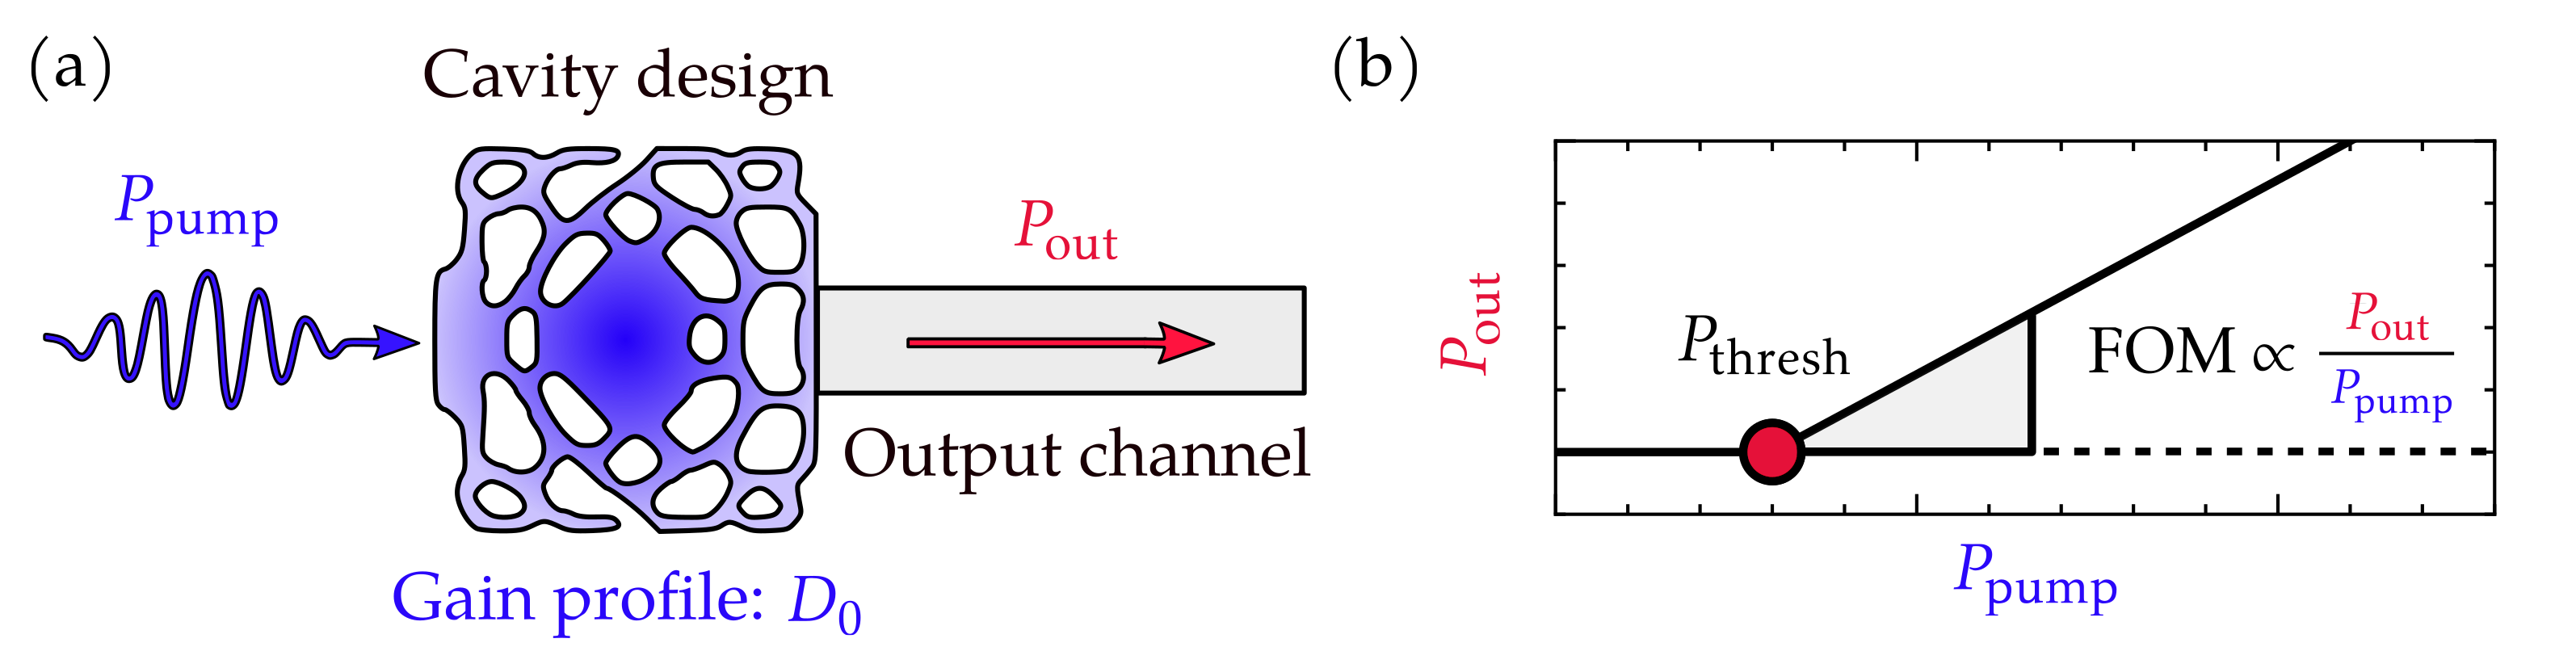
\includegraphics{figures/laser.png}}%%
    \caption{Topology optimization of nanolasers. (a) Working principle of a nanolaser. A pump with power $P_\text{pump}$ excites a gain medium with profile
    $D_0$ that emits a single lasing mode into an output channel with power $P_\text{out}$. (b) The optimization FOM is proportional to the linear relation between the pump and output power ($P_\text{out}/P_\text{pump}$),
    just above the lasing threshold ($P \gtrapprox P_\text{thres}$).  Figure adapted from~\cite{ownpub4}.}
    \label{fig:laser2d}
\end{figure}

To circumvent this, in~\cite{ownpub4}, we propose a synthesis of SPA-SALT, perturbation theory, and coupled mode theory to simplify the problem. 
The two key results of this derivation are the expression of the lasing threshold and the FOM for nanolaser design, which can be evaluated by solving a linear system of equations.
The expression for the \textbf{lasing threshold} is given by~\cite{ownpub4}
\begin{equation}\label{eq:pump_thresh}
 d_\text{thresh}  = \frac{1}{Q} \frac{\int_{\Omega} \varepsilon_c(\mathbf{r})|\mathbf{E}_{\text{r}}(\mathbf{r})|^2\, \d \Omega}{\int_{\Omega} D_0(\mathbf{r}) |\mathbf{E}_{\text{r}}(\mathbf{r})|^2\, \d \Omega}\,,
\end{equation}
where $\mathbf{E}_\text{r}$ is the field in a reciprocal problem\footnote{In a high-$Q$ system, the field from the reciprocal solve $\mathbf{E}_r$ is almost exactly equal to the cavity mode and/or the lasing mode plus a $\mathcal{O}(1/\sqrt{Q})$ error~\cite{phot_crys}.} (\eqref{eq:reciprocity}), in which the system is excited from an output port [e.g., the waveguide in \figref{fig:laser2d} (a)]. From this expression, one can reduce the lasing threshold by increasing $Q$ and enhancing the energy confinement in the
active medium. In the single-emitter limit, where an emitter located at position \(\mathbf{r}^\prime\) is modeled as 
\(D_0(\mathbf{r}) \propto \delta(\mathbf{r} - \mathbf{r}^\prime)\), 
the expression for the lasing threshold  reduces to \(d_{\text{thresh}} = V / Q\), where $V$ is a measure of the modal volume. This is a common FOM in inverse design problems outside of lasers (e.g.,~\cite{LDOS_opt_wang}) and is closely
related to the local density of states ($ \text{LDOS} \propto Q/V$)~\cite{LDOS_opt_wang}.
   Note that evaluating this lasing threshold expression (\eqref{eq:pump_thresh}) still requires solving an eigenproblem to determine \(Q\).


The second key result of the work is \textbf{a FOM for nanolaser design} that is proportional to the laser efficiency [$\propto P_\text{out}/P_\text{pump}$, \figref{fig:laser2d} (b)] and that in contrast to the lasing threshold (\eqref{eq:pump_thresh}) can be evaluated without solving an eigenproblem, through a single reciprocal solve~\cite{ownpub4}
\begin{equation}\label{eq:eff_nl}
    \frac{P_\text{out}}{P_\text{pump}} \propto \frac{\left( \int_{\Omega} D_0(\mathbf{r})|\mathbf{E}_{\text{r}}(\mathbf{r})|^2 \,  \d \Omega \right)^3} {\int_{\Omega} D_0(\mathbf{r}) |\mathbf{E}_{\text{r}}(\mathbf{r})|^4 \,  \d \Omega} = \text{FOM}.
\end{equation}
We refer to this FOM as the \emph{nonlinear} FOM, since it accounts for the laser nonlinearities perturbatively. The FOM is roughly proportional 
to the energy in the cavity ($\sim |\mathbf{E}_{\text{r}}|^6 / |\mathbf{E}_{\text{r}}|^4 \sim |\mathbf{E}_{\text{r}}|^2$), and thus to the $Q$ factor\footnote{This also contributes to attaining a low
laser threshold (\eqref{eq:pump_thresh}).}. Consequently, as the optimization progresses, the high-$Q$ assumption in SPA-SALT (\eqref{eq:SPA_SALT}) will become increasingly accurate. In the single-emitter limit, the FOM becomes
$\text{FOM}=\vert \mathbf{E}_\text{r}(\mathbf{r}^\prime) \vert^2$, which resembles an LDOS-like quantity in the reciprocal problem formulation~\cite{reci} and is proportional to the total power emitted into an output channel~\cite[App.~C]{reci}. 

To show how the nonlinear FOM compares to more conventional cavity-optimization approaches, we introduce a “naive” generalization of the LDOS, which heuristically modifies the definition
of the LDOS to account for out-coupling efficiency [through a reciprocal solve ($\mathbf{E}_r$)] and a distributed gain
medium
\begin{equation}\label{eq:SEL}
 \text{FOM}_{\text {naive }}=\int_{\Omega} D_0(\mathbf{r})\left|\mathbf{E}_{\text{r}}(\mathbf{r})\right|^2 \d \Omega\,,
\end{equation}
which we refer to as the \emph{naive} FOM, defined by the overlap of the electric-field intensity of the reciprocal field with the gain distribution.
This naive FOM is also proportional to the intensity of the reciprocal field ($\sim |\mathbf{E}_{\text{r}}|^2$), and thus roughly proportional to $Q$, and should also result in 
high-$Q$ optimized cavities. Note that this FOM also describes the case of a single-point gain region (e.g., a quantum dot),
whose location is randomly distributed in the cavity with a probability density $\mathcal{P} \sim D_0$. 

\subsection*{Optimization results for extended gain media}

\begin{figure}[tb]
    \centering
    \makebox[\textwidth][c]{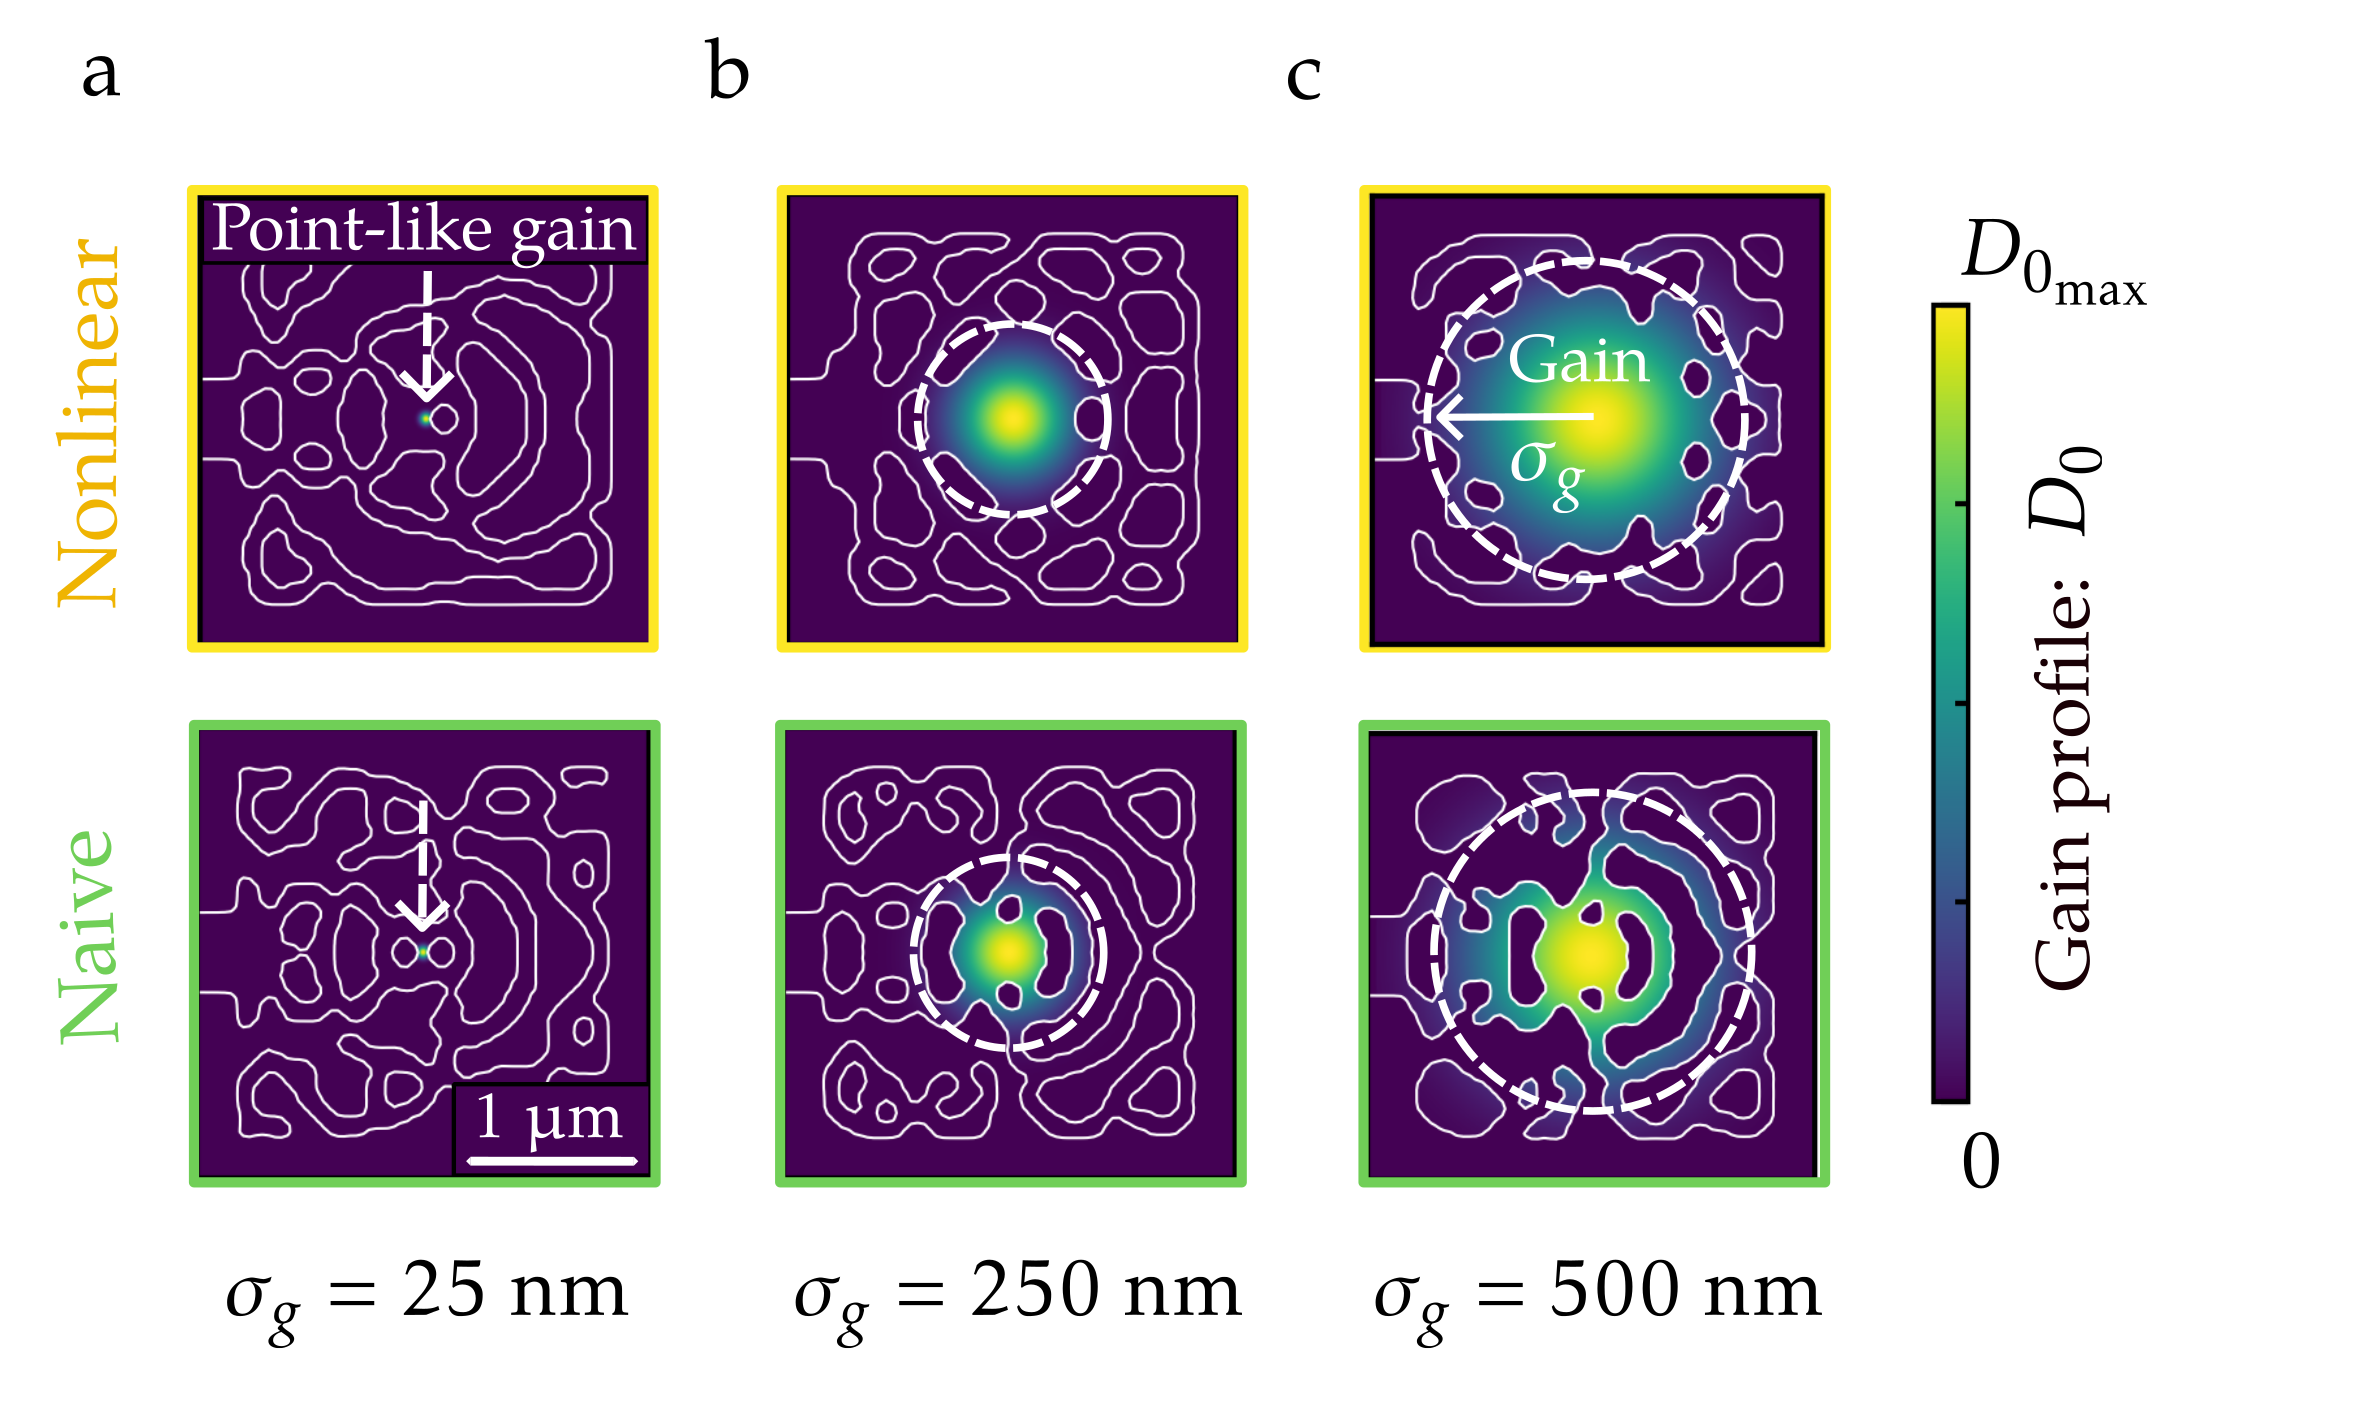
\includegraphics{figures/laser_size.png}}%%
    \caption{Topology-optimized devices when targeting the nonlinear and naive FOMs for different Gaussian gain distributions with standard deviations $\sigma_g$. (a) Device optimize for a point-like gain region ($\sigma_g=25$ nm).
    (b) Device optimized for $\sigma_g=250$ nm. (c) Device optimized for $\sigma_g=500$ nm. Figure adapted from~\cite{ownpub4}.}
    \label{fig:laser_size}
\end{figure}

Using the formalism introduced in the last subsection, we optimize two-dimensional nanolasers and study the influence of the gain region size in 
nanolaser design (\figref{fig:laser_size}). A design-dependent Gaussian distribution centered around the center, $\mathbf{r}_0$, of the cavity, describes the gain medium as
\begin{equation}
D_0 (\mathbf{r}, \hat{\rho}) = \varepsilon_{\text{r}}(\mathbf{r})  \hat{\rho}(\mathbf{r}) \, e^{- \vert \mathbf{r}- \mathbf{r}_0 \vert^2 / 2 \sigma_{\text{g}}^2 }\,,
\end{equation}
where
$\sigma_g$ is the standard deviation of the Gaussian and acts as a measure of the gain region size. We verify that for point-like gain regions, where the nonlinear and naive FOMs become equivalent, the devices optimized for the nonlinear FOM (\eqref{eq:eff_nl}) and the naive FOM (\eqref{eq:SEL})
achieve similar performance (limited by the finite size of the tiny gain region), favoring bowtie-like cavity designs
where the in-plane electric field is concentrated at a bowtie sharpness-limited field singularity~\cite{sing}. Moreover, we show that for distributed gain media with sizes comparable to the wavelength 
($\sigma_g \sim \lambda$, for $\lambda = 1.55$~\textmu m), 
the nonlinear FOM, in contrast to the naive FOM, discourages field localization due to the quartic field term in the denominator of~\eqref{eq:eff_nl} 
(since $\int |\mathbf{E}|^2$ is finite). 
This results in an approximate $3\times$ enhancement when targeting the correct (nonlinear) nanolaser FOM in~\eqref{eq:eff_nl}.

\subsection*{Accounting for gain diffusion}

In semiconductors with extended gain media, it is essential to model the electrical effect of \textbf{carrier diffusion}. This effect can be introduced by modeling the semiconductor gain medium in the free-carrier approximation\footnote{Neglecting carrier-carrier Coulomb interactions.}, using a diffusion 
equation~\cite{csalt}. Using this formalism, we re-derive the expression for the lasing threshold (\eqref{eq:pump_thresh}) when accounting for carrier diffusion effects~\cite{ownpub4}, which gives
\begin{equation}\label{eq:pump_thresh_diff}
 d_\text{thresh} = \frac{1}{Q} \frac{\int_{\Omega} \varepsilon_c(\mathbf{r})|\mathbf{E}_{\text{m}}(\mathbf{r})|^2\, \d \Omega}{\int_{\Omega} \mathcal{S} [D_0] (\mathbf{r}) |\mathbf{E}_{\text{m}}(\mathbf{r})|^2\, \d \Omega}\,,
\end{equation}
and the nanolaser FOM (\eqref{eq:eff_nl}) with carrier diffusion effects, which yields
\begin{equation}\label{eq:eff_diff}
 \text{FOM} =  \frac{\left(\int_{\Omega} \mathcal{S} [D_0](\mathbf{r}) |\mathbf{E}_{\text{r}}(\mathbf{r})|^2 \, \d \Omega\right)^3} {\int_{\Omega} \mathcal{S}\left[ |\mathbf{E}_{\text{r}}|^2\, \mathcal{S} [D_0] \right] (\mathbf{r})|\mathbf{E}_{\text{r}}(\mathbf{r})|^2 \, \d \Omega}\,.
\end{equation}
These expressions use the diffusion operator $\mathcal{S}^{-1}[\square]= \mathcal{I}\cdot\square+\nabla \cdot (R_\nabla^2\cdot \nabla \square )$, where $\square$ is a scalar field, $\mathcal{I}$ is the identity operator, and $R_\nabla (\mathbf{r})$ is a design-dependent diffusion lengthscale.
In this notation, computing $u = \mathcal{S}[b]$ corresponds to solving for the scalar field $u$ in the diffusion problem $\mathcal{S}^{-1}[u]=b$, where $b$ is a scalar field. 
The main difference when accounting for diffusion is that now one needs to consider the profile of diffused carriers ($\mathcal{S} [D_0]$) in the lasing threshold (\eqref{eq:pump_thresh_diff}), and the diffusion of the gain depletion ($\mathcal{S}[ |\mathbf{E}_{\text{r}}|^2\, \mathcal{S} [D_0]]$)
in the FOM denominator (\eqref{eq:eff_diff}). Note that in the small diffusion limit ($R_\nabla \ll \lambda, \mathcal{S} \approx \mathcal{I}$)
we recover the original expressions in \eqref{eq:pump_thresh} and \eqref{eq:eff_nl}.

\begin{figure}[tb]
    \centering
    \makebox[\textwidth][c]{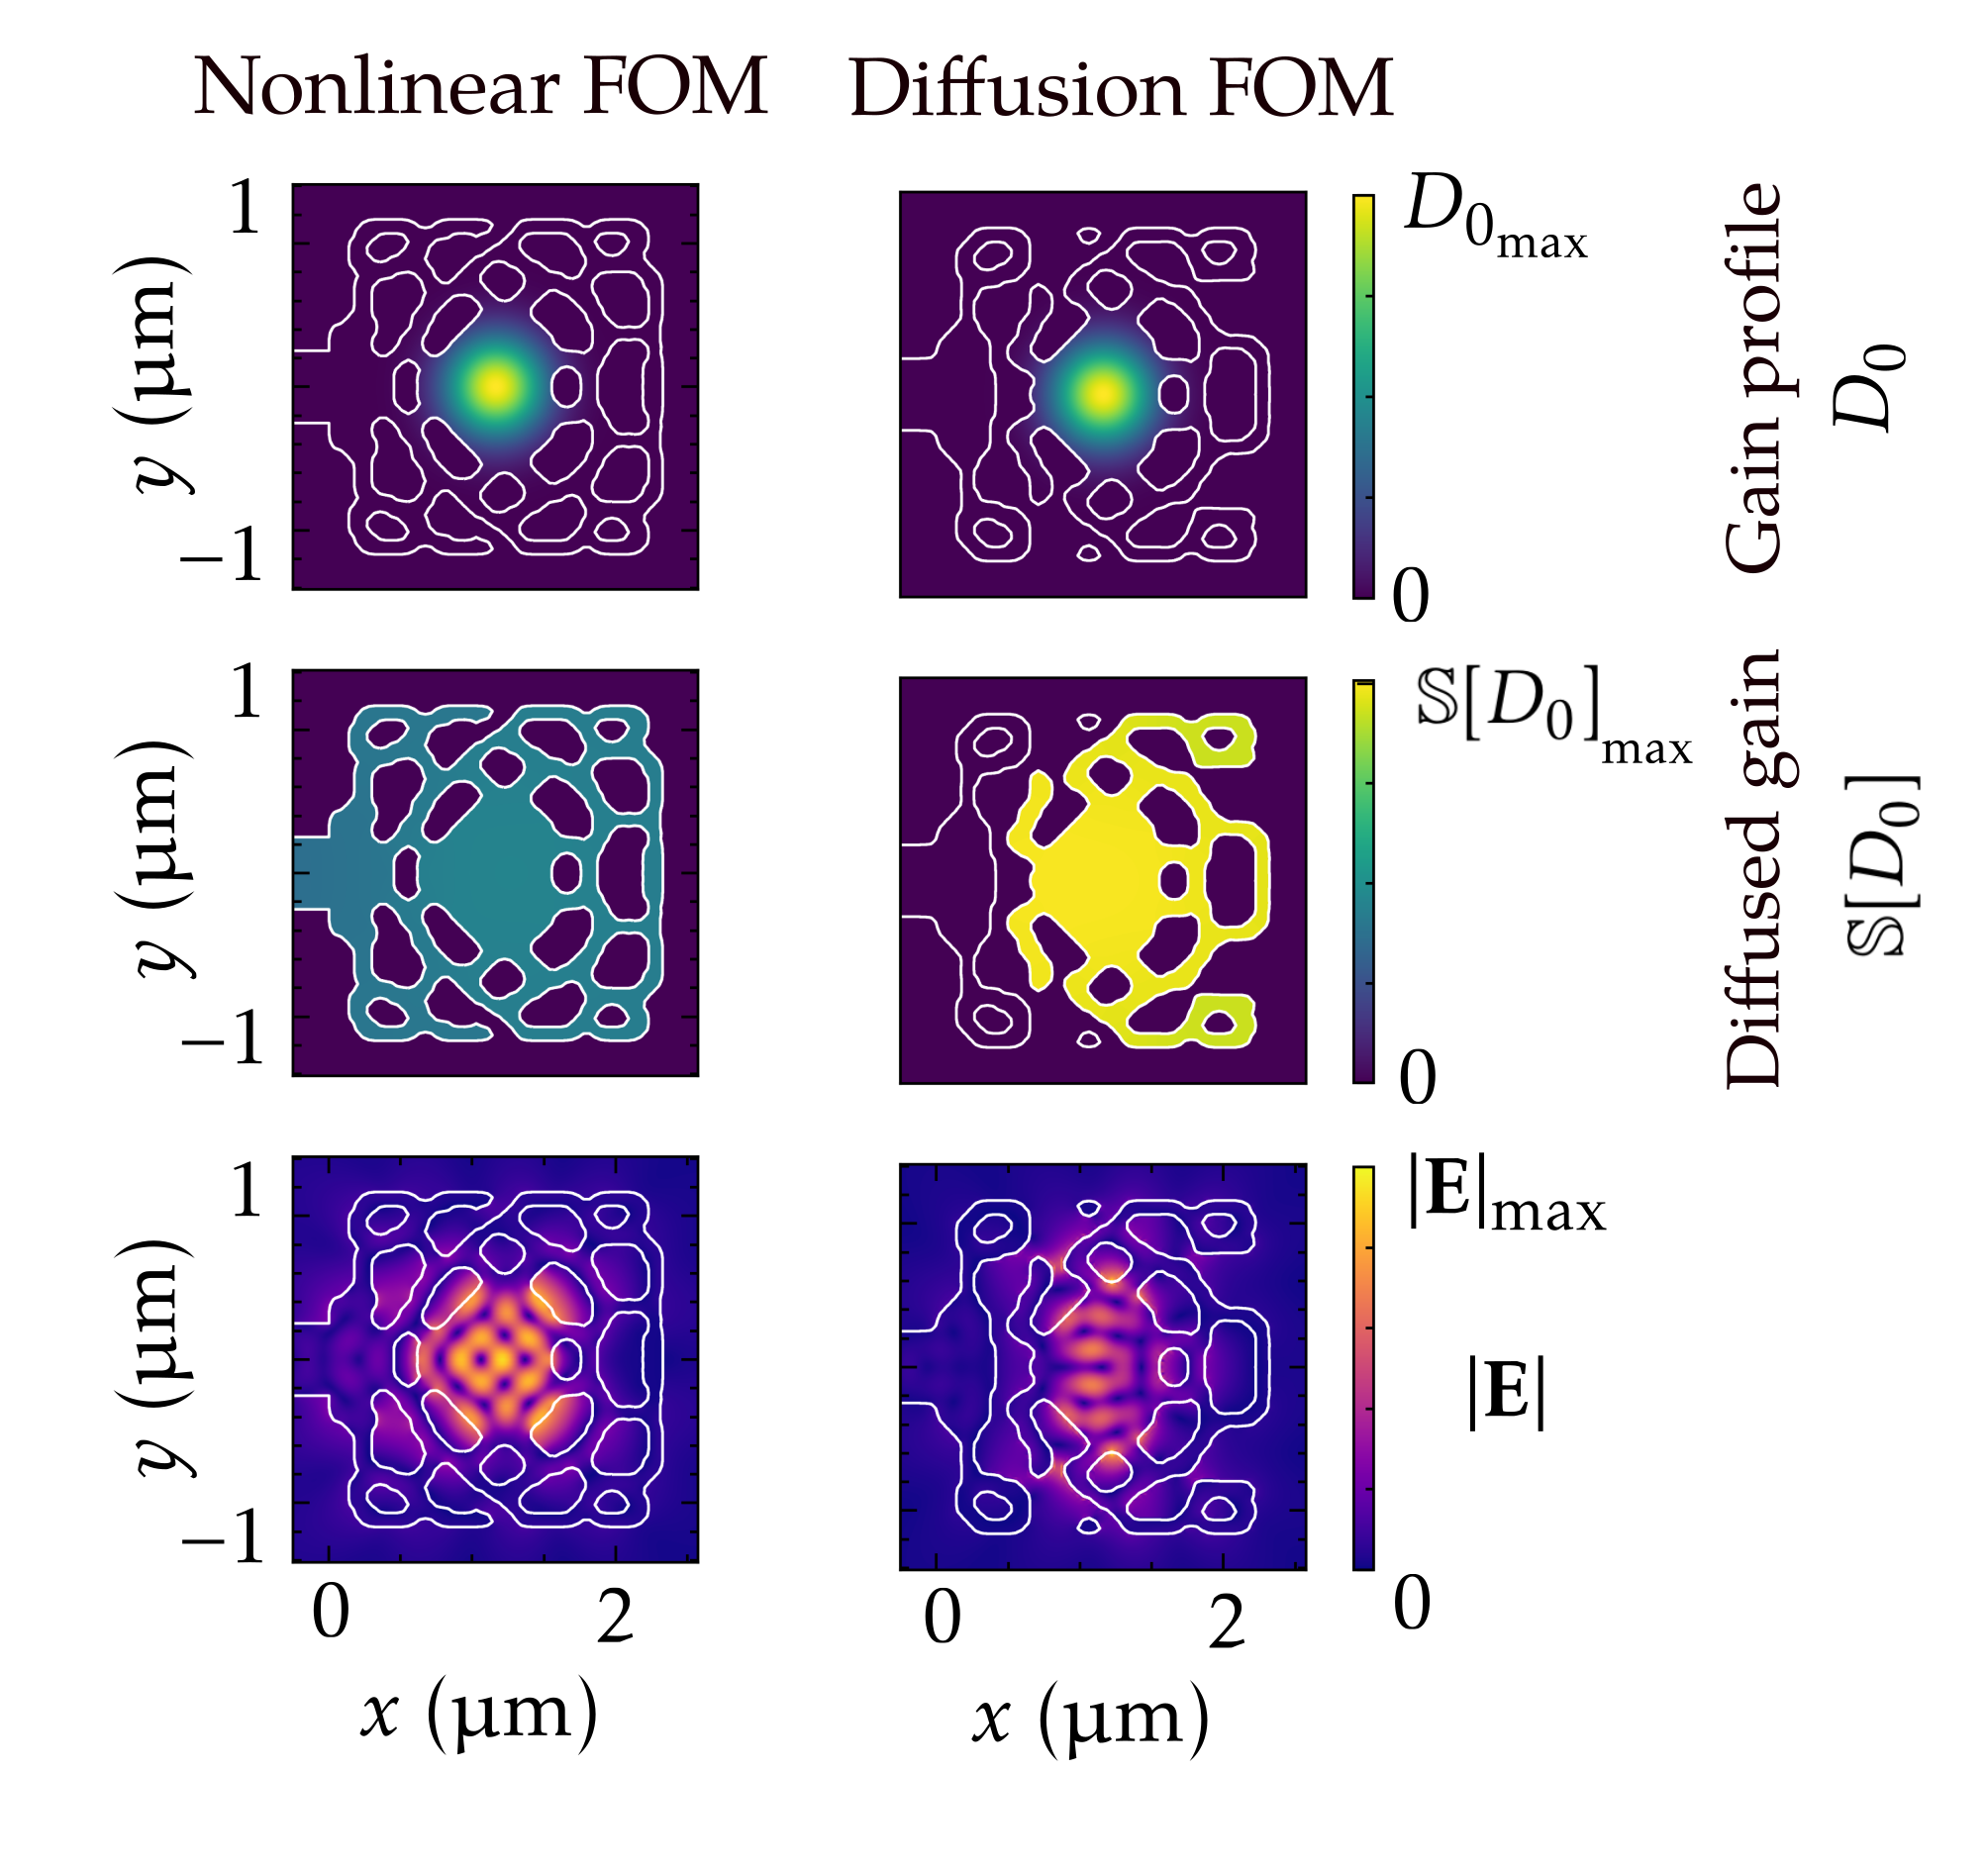
\includegraphics{figures/laser_carriers.png}}%%
    \caption{Topology-optimized devices with gain diffusion effects for a gain region with size $\sigma_g=250$ nm and a diffusion length of $R_\nabla=5$ \textmu m. The device optimized without accounting for gain diffusion ("Nonlinear FOM") and the device optimized accounting for gain diffusion ("Diffusion FOM") have the gain profile $D_0$ that is diffused ($\mathcal{S}[D_0]$)
    in the semiconductor-like material, and generate the optical field given by the electric-field norm $\vert \mathbf{E} \vert$. Figure adapted from~\cite{ownpub4}.}
    \label{fig:laser_diff}
\end{figure}

By using the expression in \eqref{eq:eff_diff} as an optimization FOM, we study how accounting for diffusion
affects the design and performance of nanolasers. As shown in \figref{fig:laser_diff}, the device that accounts for diffusion disconnects the cavity from the waveguide while also removing
material from areas of weak electric field to 
enhance the coupling between the carriers and the optical field, and results in a $\approx 2\times$ enhancement when considering the diffusion-corrected FOM. 

\subsection*{Towards realizable nanolasers: three-dimensional designs}

Finally, we apply the formalism to design three-dimensional silicon-on-insulator nanolasers (\figref{fig:laser3d}). 
We verify that, similar to the two-dimensional case, the FOM discourages field localization while still efficiently coupling to the output waveguide, yielding a $\approx 1.6\times$
enhancement when considering the correct nonlinear FOM for extended gain media (\eqref{eq:eff_nl}). We attribute the enhancement drop with respect to the two-dimensional optimization results to the fact that localizing a high-$Q$ resonance is more difficult in three dimensions, due to out-of-plane radiation losses.

\begin{figure}[tb]
    \centering
    \makebox[\textwidth][c]{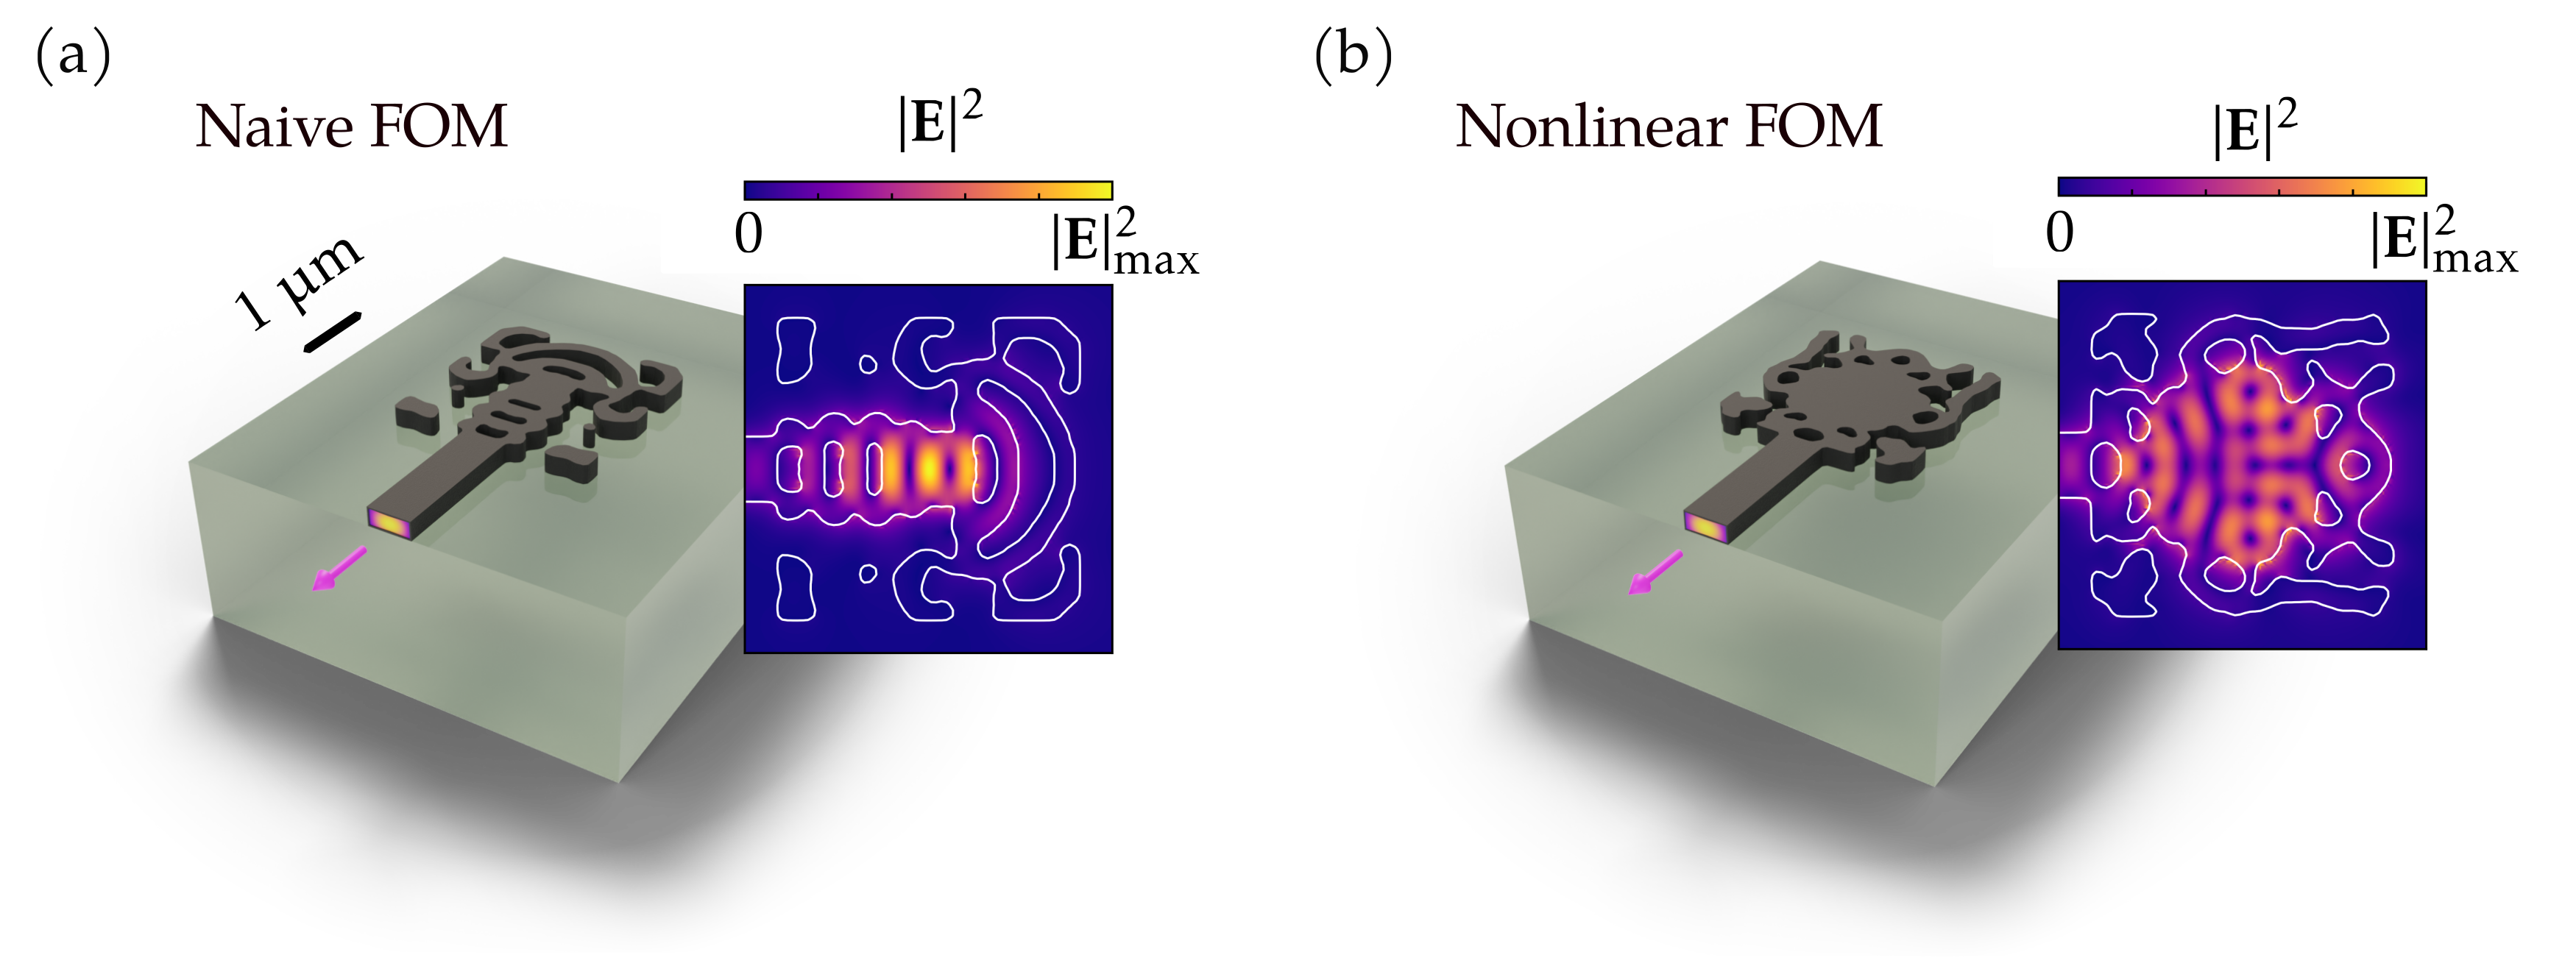
\includegraphics{figures/laser_2.png}}%%
    \caption{Topology-optimized nanolasers in three dimensions. The devices lase into the cavity mode (inset plot) and out-couple to the waveguide mode. (a) Device optimized for the naive FOM. (b) Device optimized for the nonlinear FOM.
    Figure adapted from~\cite{ownpub4}.}
    \label{fig:laser3d}
\end{figure}

\subsection*{Outlook and future work}

In conclusion, in \cite{ownpub4}, we show that by exploiting perturbative analysis valid in high-$Q$ cavities, one can derive  
an efficient FOM for laser performance ($\propto P_\text{out}/P_\text{pump}$) that, among other effects, captures resonant enhancement and gain diffusion at little extra computational cost. The FOM evaluation requires only a  
single linear reciprocal Maxwell solve (plus potentially two scalar solves for gain diffusion), making it 
an efficient formulation for laser optimization. This efficient first-principles approach allows for inverse nanolaser design in two and three dimensions, while  
also allowing for future refinements, including accounting for the laser linewidth~\cite{pick}, or accurate pumping models, where optical or electrical pumping could be explicitly
modeled by solving an additional partial differential equation.
